
\section{Theorie}
Wird in eine Schaltung mit zwei Energiespeichern, bestehend aus einer Kapazität C und einer Induktivität L, Energie hineingefühlt, fließt diese immer wieder von Speicher zu Speicher. Der daraus entstehende Schwingkreis kann über verschiedene Wege verändert werden.
\subsection{Gedämpfte Schwingungen}
Wird ein ohmscher Widerstand in den Schwingkreis eingebaut, wird elektrische Energie immer wieder in Wärme umgewandelt(\ref{fig:gedaempfter_schwingkreis}). Mit der Zeit nehmen die Amplitude von Strom und Spannung ab. 
Es wird von einer gedämpften Schwingung gesprochen.
\begin{figure}[H]
    \centering
    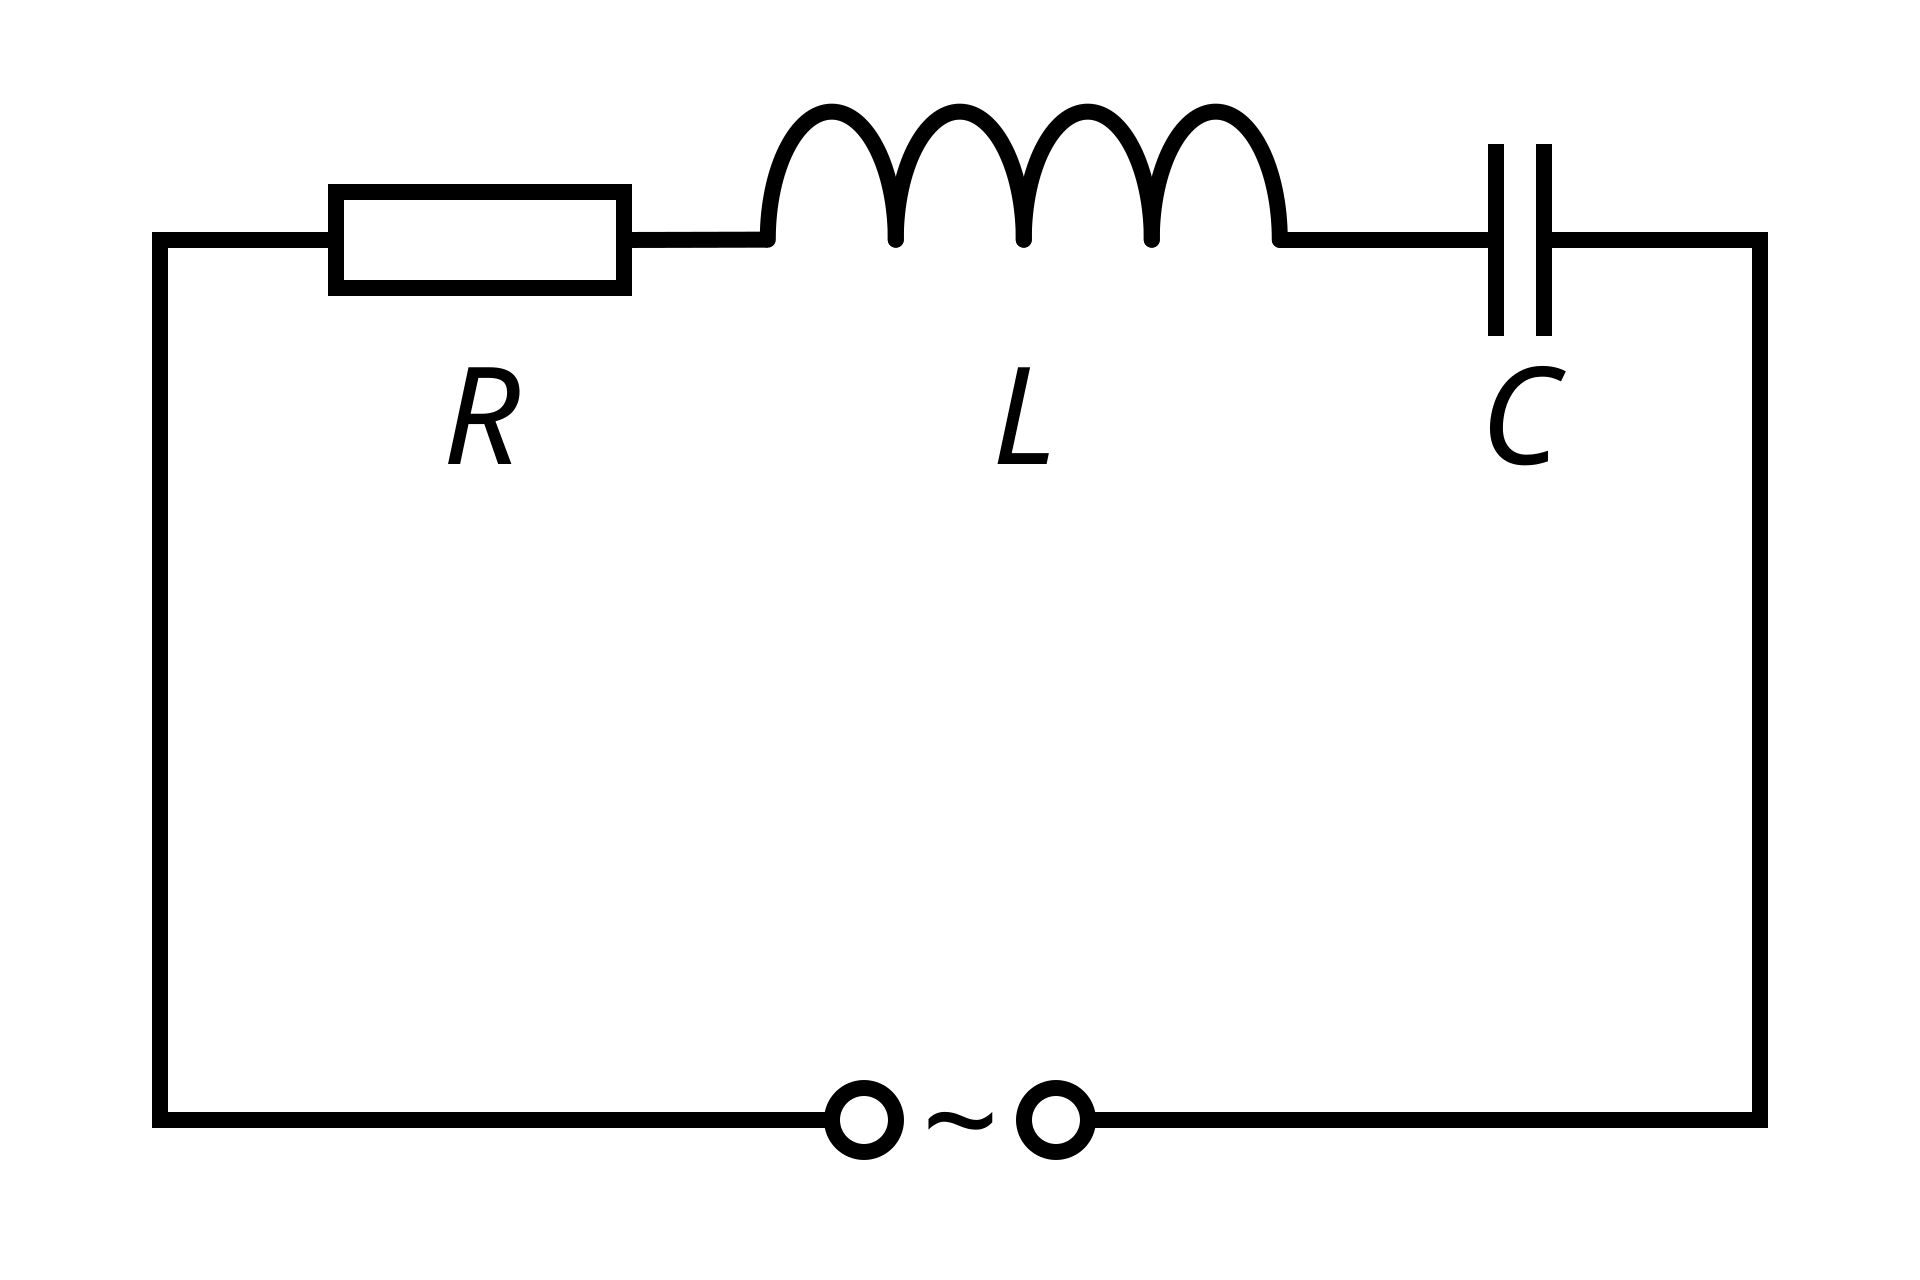
\includegraphics[width=0.5\textwidth]{Gedaempfter_Schwingkreis.png}
    \caption{Gedämpfter Schwingkreis\cite{gedaempfter_schwingkreis}}
    \label{fig:gedaempfter_schwingkreis}
\end{figure}
\subsection{Erzwungene Schwingungen}
Wird dem Schwingkreis eine zeitabhängig schwingende Spannung angelegt, schwingt der Schwingkreis mit der Frequenz der Spannung. In Abhängigkeit des Widerstands, der Kapazität und der Induktivität gibt es eine Frequenz, bei der ein Maximum an Energie in den Schwingkreis geführt werden kann. Es kommt zu einem Maximum der Stromamplitude bei dieser Resonanzfrequenz.

\subsection{Formeln}
